\chapter{Results and Performance Analysis}
\label{chapter:performance_analysis}

\section{Background Measures and Reproducible Setup}

The Classical Model calculates relative information against a minimally informative background distribution over an intrinsic range $[L,U]$. For each variable, the smallest and largest elicited bounds (and, for seed variables, the realization) define the observed range; a 10\% overshoot is added at both ends. Uniform backgrounds are used for proportions and rates (Seeds 5, 7, and 9; Target 4). Log-uniform backgrounds are used for the remaining positive scale variables. The latter assigns equal probability to equal ratios and is invariant to a change of units.

Within each background range, an expert's density is piecewise uniform (or piecewise log-uniform) over the four inter-quantile intervals with probability masses $(0.05,0.45,0.45,0.05)$. All calculations were independently reproduced in Python. The analysis validates quantile ordering, computes seed-bin counts and scores, constructs linear pools, numerically inverts each pooled cumulative distribution to obtain target quantiles, and exports the anonymous tables used below.

\section{Aggregation Schemes}

Two aggregation schemes are retained for direct comparison. The Equal Weight Decision Maker (EWDM) assigns $1/7$ to every expert. The performance-weighted Decision Maker assigns raw weight
\[
w_e=\operatorname{Cal}_e\operatorname{Inf}_e\mathbf{1}\{\operatorname{Cal}_e\geq\alpha\}
\]
and normalizes the retained weights to sum to one. The optimized threshold $\alpha^*$ is selected from the realized expert calibration scores to maximize the product of the resulting virtual expert's calibration and mean information. This comparison follows the empirical-control role of seed variables in the Classical Model~\cite{cookeGoossens2008,colsonCooke2018}.

\section{Individual Expert Performance}

Table~\ref{tab:expert_performance_results} reports the realized bin counts, statistical-accuracy score, mean information score, raw score, and optimized normalized weight. Experts 2 and 4 have the highest calibration score ($0.2441$). Experts 6 and 7 have a calibration score of only $0.0008$; both place four realizations below their 5th percentile and two above their 95th percentile, evidence of substantial miscalibration rather than merely low informativeness.

The optimization considered zero and each distinct expert calibration score as candidate cut-offs. The maximum combined Decision Maker score occurs at $\alpha^*=\OptimalAlpha$. Five experts meet this threshold. Experts 2 and 4 receive approximately 75\% of the total optimized weight, while Experts 6 and 7 receive zero. This concentration is a direct consequence of the scoring rule and is also a reason to compare the result with equal weighting rather than accepting it uncritically.

\begin{table}[htbp]
    \centering
    \scriptsize
    \begin{tabular}{lccccc}
        \toprule
        \textbf{ID} & \textbf{Bins 1--4} & \textbf{Calibration} & \textbf{Mean info.} & \textbf{Raw score} & \textbf{Weight} \\
        \midrule
        Expert 1 & 3--3--4--0 & 0.0608 & 1.107 & 0.0674 & 0.096 \\
Expert 2 & 2--5--3--0 & 0.2441 & 1.084 & 0.2645 & 0.376 \\
Expert 3 & 3--3--4--0 & 0.0608 & 1.103 & 0.0671 & 0.095 \\
Expert 4 & 2--5--3--0 & 0.2441 & 1.082 & 0.2642 & 0.376 \\
Expert 5 & 3--2--5--0 & 0.0357 & 1.118 & 0.0400 & 0.057 \\
Expert 6 & 4--3--1--2 & 0.0008 & 0.983 & 0.0008 & 0.000 \\
Expert 7 & 4--1--3--2 & 0.0008 & 1.073 & 0.0009 & 0.000 \\
\bottomrule

    \end{tabular}
    \caption{Empirical scores and optimized weights. Bin counts correspond to intervals below the 5th, between the 5th and 50th, between the 50th and 95th, and above the 95th percentile.}
    \label{tab:expert_performance_results}
\end{table}

\section{Decision Maker Performance}

Table~\ref{tab:dm_performance} compares the virtual experts on the same seed variables. The equal-weight DM is more statistically accurate, but substantially less informative. The optimized DM has the higher product score ($0.2988$ versus $0.2191$), so it is selected for the primary forecasts. The equal-weight results remain visible in Chapter~\ref{chapter:results} as a robustness benchmark.

\begin{table}[htbp]
    \centering
    \begin{tabular}{lccc}
        \toprule
        \textbf{Decision Maker} & \textbf{Calibration} & \textbf{Mean information} & \textbf{Combined score} \\
        \midrule
        Equal-weight DM & 0.6828 & 0.321 & 0.2191 \\
Optimized performance-weight DM & 0.3005 & 0.994 & 0.2988 \\
\bottomrule

    \end{tabular}
    \caption{Performance of the equal-weight and optimized Decision Makers on the seed variables.}
    \label{tab:dm_performance}
\end{table}

The distinction matters: calibration and information reward different properties. Equal weighting produces wider distributions that cover the realizations more often, whereas optimized performance weighting retains sharper distributions while remaining acceptably calibrated. Selecting the optimized DM is therefore supported by the proper combined score, not by informativeness alone.

Figure~\ref{fig:expert_performance} visualizes the trade-off. Marker area represents optimized weight. Experts 2 and 4 occupy the high-calibration region and consequently dominate the pool; Experts 6 and 7 fall well to the left of the selected threshold.

\begin{figure}[htbp]
    \centering
    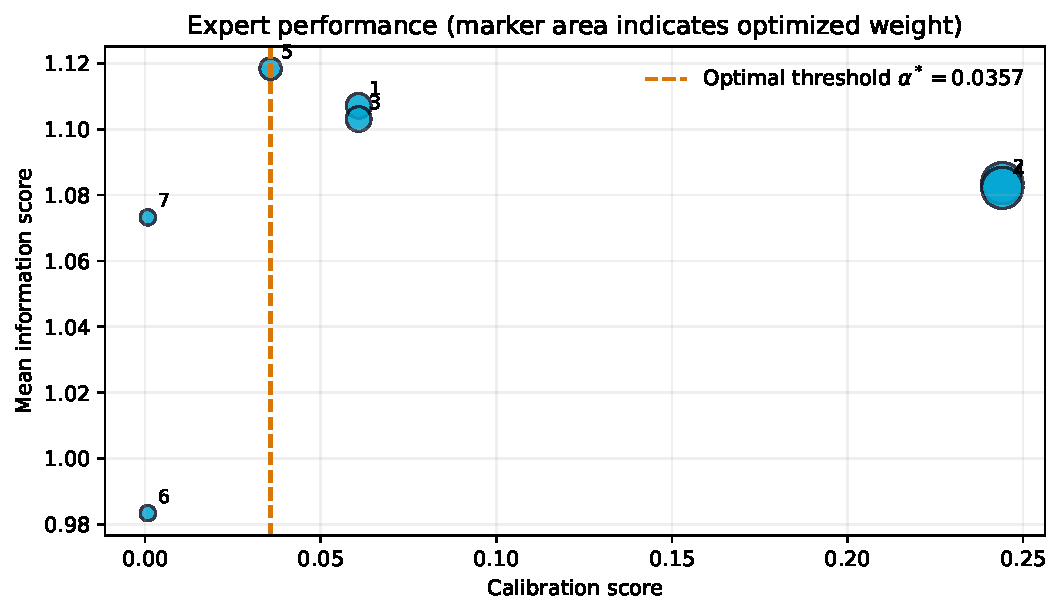
\includegraphics[width=0.82\textwidth]{figures/generated/expert-performance.pdf}
    \caption{Calibration and mean information scores for the seven experts. Labels are anonymous expert identifiers; marker area is proportional to optimized weight.}
    \label{fig:expert_performance}
\end{figure}
